% chapitre de description du travail technique
\chapter{Technical work}

\label{technic}




\definecolor{mygreen}{RGB}{28,172,0} % color values Red, Green, Blue
\definecolor{mylilas}{RGB}{170,55,241}

\lstset{language=Matlab,%
    %basicstyle=\color{red},
    breaklines=true,%
    morekeywords={matlab2tikz},
    keywordstyle=\color{blue},%
    morekeywords=[2]{1}, keywordstyle=[2]{\color{black}},
    identifierstyle=\color{black},%
    stringstyle=\color{mylilas},
    commentstyle=\color{mygreen},%
    showstringspaces=false,%without this there will be a symbol in the places where there is a space
    numbers=left,%
    numberstyle={\tiny \color{black}},% size of the numbers
    numbersep=9pt, % this defines how far the numbers are from the text
    emph=[1]{for,end,break},emphstyle=[1]\color{red}, %some words to emphasise
    %emph=[2]{word1,word2}, emphstyle=[2]{style},
}

%---------------------

\section{Code Refactoring}
When working with new code, the first thing to do is to understand it. Then, you must do the necessary modifications.
\subsection{Understanding the code}
When I arrived at IRI, another student was already working on applying particle filtering on a robot simulation.
He was doing his third-year internship and was working at the IRI since March. He based his work on Mr Jaulin's latest research: \parencite{Base}.
%describe and expand

When first discovered, the code was mainly organized in three parts:
\begin{itemize}
  \item The Interval class
  \item The Box particle filtering
  \item The Main
\end{itemize}
\subsubsection{The Interval Class}
The interval class was directly inspired by Mr Jaulin's works and courses \parencite{IAMOOC}.
It's a simple class enabling the use of Interval analysis in Matlab, by creating a new object, and overloading the standard comparators and operators.\\

As such, this new object is in fact defined by a couple upper bound and lower bound for each dimension we are in.
In this case, the simulation we work on is two dimensional, so the intervals have two bounds of each kind.
\subsubsection{The Box particle filtering}
"Resulting from the synergy between the sequential Monte Carlo method and interval analysis, box particle filtering is an approach that has recently emerged and is aimed at solving a general class of nonlinear filtering problems.
This approach is particularly appealing in practical situations involving imprecise stochastic measurements that result in very broad posterior densities.\\

It relies on the concept of a box particle that occupies a small and controllable rectangular region having a nonzero volume in the state space.
Key advantages of the box particle filter against the standard particle filter are its reduced computational complexity and its suitability for distributed filtering.\\

Indeed, in some applications where the sampling importance resampling PF may require thousands of particles to achieve accurate and reliable performance, the box-PF can reach the same level of accuracy with just a few dozen box particles."\parencite{BPF}

As seen, the BPF is an efficient filter in our case. Aimed mainly at imprecise measurements, and using interval analysis, it integrates perfectly with what we are looking for.

\subsubsection{The Main}
Two more files are used in the program.\\

In the environment file, all the variables needed at the start of the program,
 such as the trajectory, the number of boxes, or the length of the simulation are defined.\\

The Mainbox file is simply the main loop, and the one where the graphical interface is created. It's no more than printing the trajectories for the real and the self-perceived bots.

\subsection{Changing the way it works}
The first thing to do was to change completely how the main loop worked.
The new system needed to be robust, simple and calculate step after step.\\

\begin{figure}[ht]
\centering
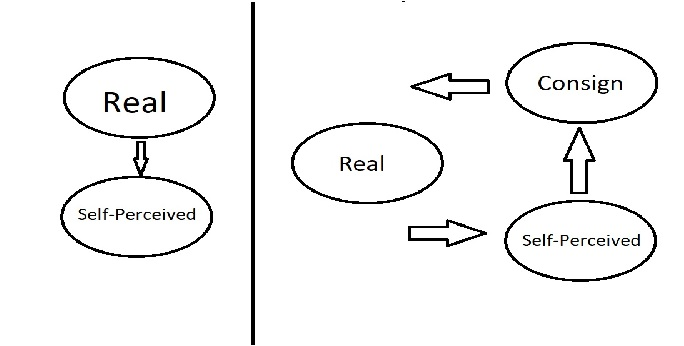
\includegraphics{Figures/Loops}
\decoRule
\caption[Direct and controled loops]{How the new control loop was implemented.}
\label{fig:Loops}
\end{figure}

In the first program, the point of interest was measuring the position and the speed of the robot.
The system had no feedback loop, so there was no need to calculate step by step. All the calculation for the robot's position and movement were done before the program's actual work began.
The new feedback loop needed all the parameters from a step to calculate the next one.\\

Information from the consign trajectory and the self-perceived robot were used to calculate the real position of the robot.
The real position was then used to infer the new self-perceived position, feeding the loop again.
As seen in Figure \ref{fig:Loops}, this adds a level of complexity to the program.\\

From one point to another, the system had many calculations to do, primarily due to the BPF.
Indeed, the BPF is a system which needs a lot of diverse points to operate efficiently. A sample size of 2000 points was sometimes reached.
My feedback loop and control system needed to be light and fast, or it would have slowed the program even more.\\


\section{Simple control}
After the new loop was added, I had to modify the informations sent from one part of the loop to another.

\subsection{Adding precision}
Before the work on control algorithm started, I had discovered that the information returned by the BPF were much more precise than simply using the sensor's feed, but consistency was lacking.
Indeed, from one step to another, the BPF could render highly different results, and it would cause the real robot behaving erratically.
To compensate, a low-pass filter was added, by using a sliding median of the last five values instead of only the last one.\\

Although such a system means that the correction is a bit late, it suppresses most of the erratic behaviour from the self-perceived bot.
Giving more weight to the last value was tested, but the erratic behaviour came back with too much force, so the idea was dropped.
More tests were made with a sliding median on more or less values, but five was the best compromise.
The system was only around two steps late, so about 1/10th of a second.\\

This kind of treatment is often used on real robots.
Usually, sensors have a high communication rate (around 500Hz for an IMU) whereas actuator control board work around 10Hz.
That kind of differences means that, on real robots, sudden spikes and outliers from sensors can be minimized without impacting the rate of information sent to actuators.
Sadly, on this simulation, the sensor rate was limited by the BPF calculation rate.
Eventually, I used a sliding median, but the trade-off was the slight lateness of the control algorithm.\\

\subsection{Testing methods and taking control}

The new loop, at the beginning, did nothing more than transmitting information from one part of the program to another.
At first, a simple proportional control was added. A divergence from the original trajectory was met by a correction proportional to the deviation.

This system was too unstable or too slow.
As it is often the case for proportional control, the bot would either overshoot, or not be able to reach the designated trajectory.\\

The next step was using a proportional derivative method. This solved the overshoot problems I had, and the corrections were much faster.
This system was based on a feedback linearization, as described in \parencite{ROBMOOC}.
It was implemented in a simple way, by adding a control variable named U.\\

{\small
\begin{lstlisting}[caption=Control Code, label=controlcode, frame=single]
function u = control(x,w,dw)
%control : creates consign vector from state and trajectory vector
    A = [-x(4)*sin(x(3)), cos(x(3));
         x(4)*cos(x(3)), sin(x(3)) ];
    Y = [x(1); x(2)];
    dY= [x(4)*cos(x(3));x(4)*sin(x(3))];
    V = (w-Y)+2*(dw-dY);
    u = A\V;
end
\end{lstlisting}
}


In this code, we suppose the existence of a nonlinear system described by:\\

\begin{equation}
\left \{
\begin{array}{r c l}
   \dot{x} & = & f(x) + g(x)u \\
   y & = & h(x)
\end{array}
\right .
\end{equation}

This system describes the movements of our simulated robot. By differenciating $y_i$ until inputs are involved inthe expression of the derivative, we obtain:

\begin{equation}
  \begin{pmatrix}
    y_{1}^{(k_1)} \\
    \vdots \\
    y_{m}^{(k_m)}
  \end{pmatrix}
  = A(x)u + b(x)
\end{equation}

If we suppose that $A$ is invertible, we can write:

\begin{equation}
  \label{eq2}
  u = A^{-1}(x)(v - b(x))
\end{equation}

Thus, going back to the code \ref{controlcode}, each member of the equation \ref{eq2} can be joined with the similarly named variable in the code.\\

Once the control loop has been established, we need to add it in a main loop.

The Main loop in this program is copied here :\\

{\small
\begin{lstlisting}[frame=single]
for k=1:N
    %display iteration number
    disp(k);
    %create control vector
    % xc,dxc,ddxc,vc,thetac : full state of consign robot (position,
    % derivative, second derivative, speed, and angle)
    [xc,dxc,ddxc,vc,thetac]=consigne(k,ts);
    ur=control([x_med2 theta_measure v_measure],xc,dxc);
    %new step for the state of the system
    [x,v,theta,v_measure, theta_measure, pe, U]=realState(N, x, v, theta,ur, ts,S,NS);
    %box particle filtering
    [w_box_1,w_box_2,x_med] = Boxfilter1(Boxes,ts,stateF,U,pe,w_boxes{k});
    x_med_box(k,:)=x_med;
    w_boxes{k}=w_box_1;
    w_boxes{k+1}=w_box_2;
    %low pass filter (gliding median) on median position from BPF
    if k>5
        x_med2=sum(x_med_box(k-5:k,:))/5;
    else
        x_med2=x_med;
    end
    %creating positions of real, self-measured and consign robots
    x_tank=[x(1);x(2);theta]; % real robot
    xm_tank=[x_med2(1);x_med2(2);theta_measure]; %measured robot
    xc_tank=[xc; thetac]; %consign robot
    %saving those positions in lists.
    x_tank_list(:,k)=x_tank;
    xm_tank_list(:,k)=xm_tank;
    xc_tank_list(:,k)=xc_tank;
end
\end{lstlisting}
}


As seen in this code, each step of trajectory calculation is immediately followed by a step of BPF on the information given by the simulated sensors. \\


As a side note, I also tried to adapt a H-infinity control method, but a few problems blocked my way.
The more evident one was that the model I used was far from enough for this method to yield good results.
And of course, the use of a BPF resulted sometimes in singularities or in a kind of saturation that rendered the method completely unusable.


\section{Obstacle Avoidance}
Now that the robot was able to follow a trajectory, with more or less success, depending on the precision reached by the BPF, it needed to avoid obstacles and walls.


\subsection{Trials and errors}

One of the best ways to avoid obstacles in a partially known environment is a vector field.
In my case, I had to add the right vector to the vector I had already created with the control system.\\

My first try was simply by adding repulsive vectors stemming from boxes colliding with a wall.
This test was far from successful, since the self-perceived robot, a bit late because of the low-pass filter, would often make a U-turn, and completely lose itself.
Indeed, the vector field, radiating only from colliding boxes, would overrun the control vector and push back the robot until the robot was far enough from the consign for shenanigans to ensue.

I then tried to use various parts of the map, first creating a single vector, then with multiple vectors, but I then determined that I had to use the whole known surroundings.

\subsection{Creating a vector field}
\label{vectf}

I had to devise a way for the robot to be aware of his surroundings as a whole.\\

{\small
\begin{lstlisting}[caption=Vector Field, frame=single]
function [Mx,My] = fieldmat(envimat,k)
%% fieldmat : creates two vector fields, acting as repulse fields from the walls.
% - Inputs=
%   -envimat - DOUBLE ARRAY, environement matrix
%   -k - optional - DOUBLE, strength of the vector field
% - Outputs =
%   -Mx - DOUBLE ARRAY, matrix of the x-axis part of the vector field
%   -My - DOUBLE ARRAY, matrix of the y-axis part of the vector field
    if (exist('k')==0), k=12; end;
    [m,n]=size(envimat);
    walls=envimat==ones(m,n);
    free=envimat==2*ones(m,n);
    Mx=zeros(m,n);
    My=zeros(m,n);
    Mx(:,1)=k;
    Mx(:,end)=-k;
    My(1,:)=k;
    My(end,:)=-k;
    for i=2:m-1
        for j=2:n-1
            Mx(i,j)=k*(walls(i,j-1)-walls(i,j+1));
            My(i,j)=k*(walls(i-1,j)-walls(i+1,j));
        end
    end
    Mx=imgaussfilt(Mx,5).*walls+imgaussfilt(Mx,3).*free;
    My=imgaussfilt(My,5).*walls+imgaussfilt(My,3).*free;
\end{lstlisting}
}


I created a small sub-program able to infer a repulsive vector field from an image of the obstacles.\\

\begin{figure}[H]
\centering
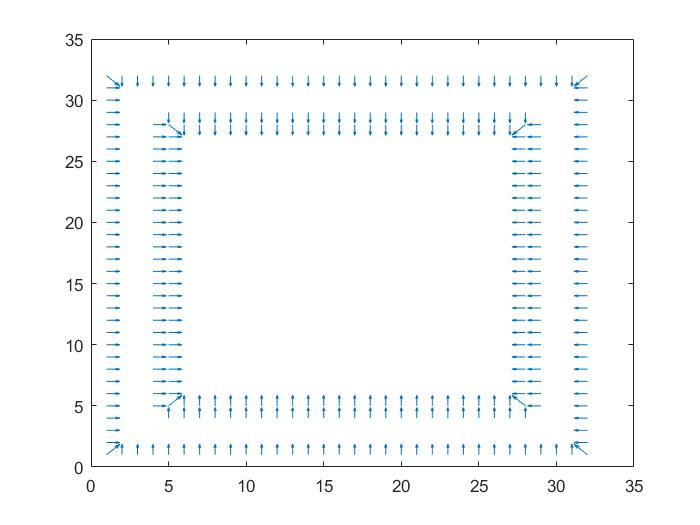
\includegraphics[scale=0.4]{Figures/quiver1}
\decoRule
\caption[Basic Quiver]{Quiver of basic vector field created from the obstacles.}
\label{fig:quiver1}
\end{figure}


 This program has two parts. First, a repulsive vector is added in each box next to an obstacle.
 This creates a series of vectors each of equal power, as seen in Figure \ref{fig:quiver1}.\\

 \begin{figure}[H]
 \centering
 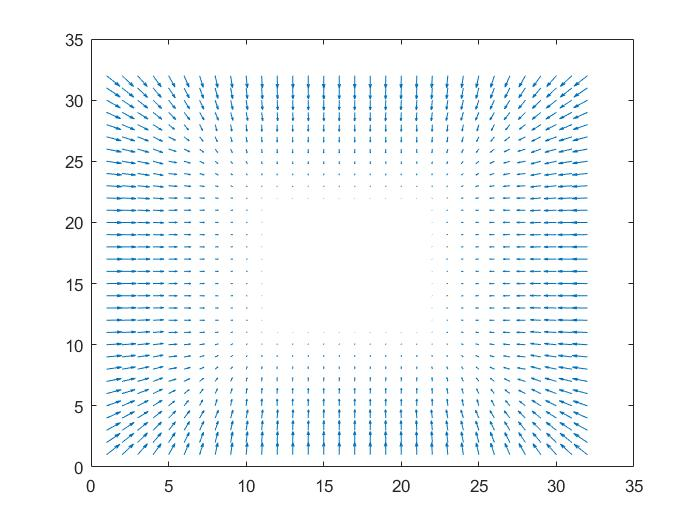
\includegraphics[scale=0.4]{Figures/quiver2}
 \decoRule
 \caption[Blurred Quiver]{Gaussian blur added to the first vector field.}
 \label{fig:quiver2}
 \end{figure}

 After that, a gaussian blur is added to the matrix, using a bigger parameter on the obstacle parts than on the free parts of the playground.
 This ensures that, if the self-perceived robot gets in an obstacle, it will be met by a stronger repulsive force.
 The result of the blur can be seen on Figure \ref{fig:quiver2}\\



%{\small
\begin{lstlisting}[caption=Vector Field, frame=single]
function [Mx,My] = fieldmat(envimat,k)
%% fieldmat : creates two vector fields, acting as repulse fields from the walls.
% - Inputs=
%   -envimat - DOUBLE ARRAY, environement matrix
%   -k - optional - DOUBLE, strength of the vector field
% - Outputs =
%   -Mx - DOUBLE ARRAY, matrix of the x-axis part of the vector field
%   -My - DOUBLE ARRAY, matrix of the y-axis part of the vector field
    if (exist('k')==0), k=12; end;
    [m,n]=size(envimat);
    walls=envimat==ones(m,n);
    free=envimat==2*ones(m,n);
    Mx=zeros(m,n);
    My=zeros(m,n);
    Mx(:,1)=k;
    Mx(:,end)=-k;
    My(1,:)=k;
    My(end,:)=-k;
    for i=2:m-1
        for j=2:n-1
            Mx(i,j)=k*(walls(i,j-1)-walls(i,j+1));
            My(i,j)=k*(walls(i-1,j)-walls(i+1,j));
        end
    end
    Mx=imgaussfilt(Mx,5).*walls+imgaussfilt(Mx,3).*free;
    My=imgaussfilt(My,5).*walls+imgaussfilt(My,3).*free;
\end{lstlisting}
}


\section{Graphic User Interface}

Since my work was a bit tedious on something so dry, I decided to add a graphical interface.

\subsection{Adding an interface}

In this interface, I decided first to add the choice to show each component separately. Checkboxes enable the visualisation of the robot, the environment, the boxes or the landmarks.
Those choices will be reflected on the visualisation after clicking on show.\\

The simulation length and the percentile of boxes shown can be adjusted via two sliders.
Those are useful to mitigate the precision of the simulation with the time spent on calculations.\\

\begin{figure}[H]
\centering
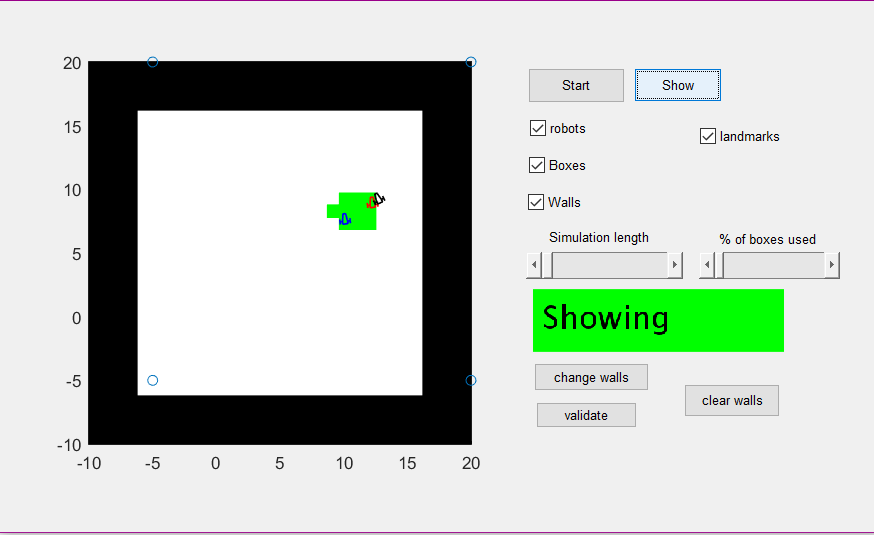
\includegraphics[scale=0.7]{Figures/Gui}
\decoRule
\caption[Gui]{Full GUI for the algorithm}
\label{fig:gui}
\end{figure}

Part of the challenge of the algorithm was to make it reliable enough for it to run in any environment.
I then added a graphical way to change the place of the obstacles, to test the program in all the possibilities.
It did prove quite useful, since it was how the vector field coefficients were adjusted.


\subsection{The full program}

The program is now organized in four parts:
\begin{itemize}
  \item the BPF
  \item the Interval class
  \item the Vector field
  \item the GUI
\end{itemize}
Even though the first two have the same inner workings than at the beginning, the last two are new.

\subsubsection{the Vector field}

As mentioned in \ref{vectf}, a subprogram was added to create the necessary vector field.
This program can be called at any moment, and will create a vector field with any size of matrix.
If the size of the playground or the boxes changes, this program will still be able to work.

\subsubsection{the GUI}

Due to Matlab's way, the new main is simple.m, the file containing the GUI description.
Part of the Main was tranferred in this new file, and part of the envionment file can now also be found there.\\

This is due to the variables that can be adjusted in the GUI.
A lot of variables were also duplicated in handles, because those were used in multiple parts of the program, and had to be transferred from one part to another.
